%% homology_orthology_paralogy.tex
%% Author: Leighton Pritchard
%% Copyright: James Hutton Institute
%% A brief description of the -logues

% SUBSECTION: Genome Features
\subsection{Who let the -logues out?}

% ncRNA features
\begin{frame}
  \frametitle{Who let the -logues out?\footnote{\tiny{Fitch (2000) \textit{Trends Genet.} \textbf{16}:227-231 \href{http://dx.doi.org/10.1016/S0168-9525(00)02005-9}{doi:10.1016/S0168-9525(00)02005-9}}}}
    \begin{itemize}
      \item \textbf{homologues}: elements that are similar because they share a common ancestor. \textbf{There are NOT degrees of homology}
      \item \textbf{analogues}: elements that are (functionally?) similar, and this may be through common ancestry \textit{or} some other means, e.g. convergent evolution
      \item \textbf{orthologues}: homologues that diverged through speciation
      \item \textbf{paralogues}: homologues that diverged through duplication within the same genome
    \end{itemize}
\end{frame}

% Regulatory features
\begin{frame}
  \frametitle{Who let the -logues out?}
  \begin{center}
    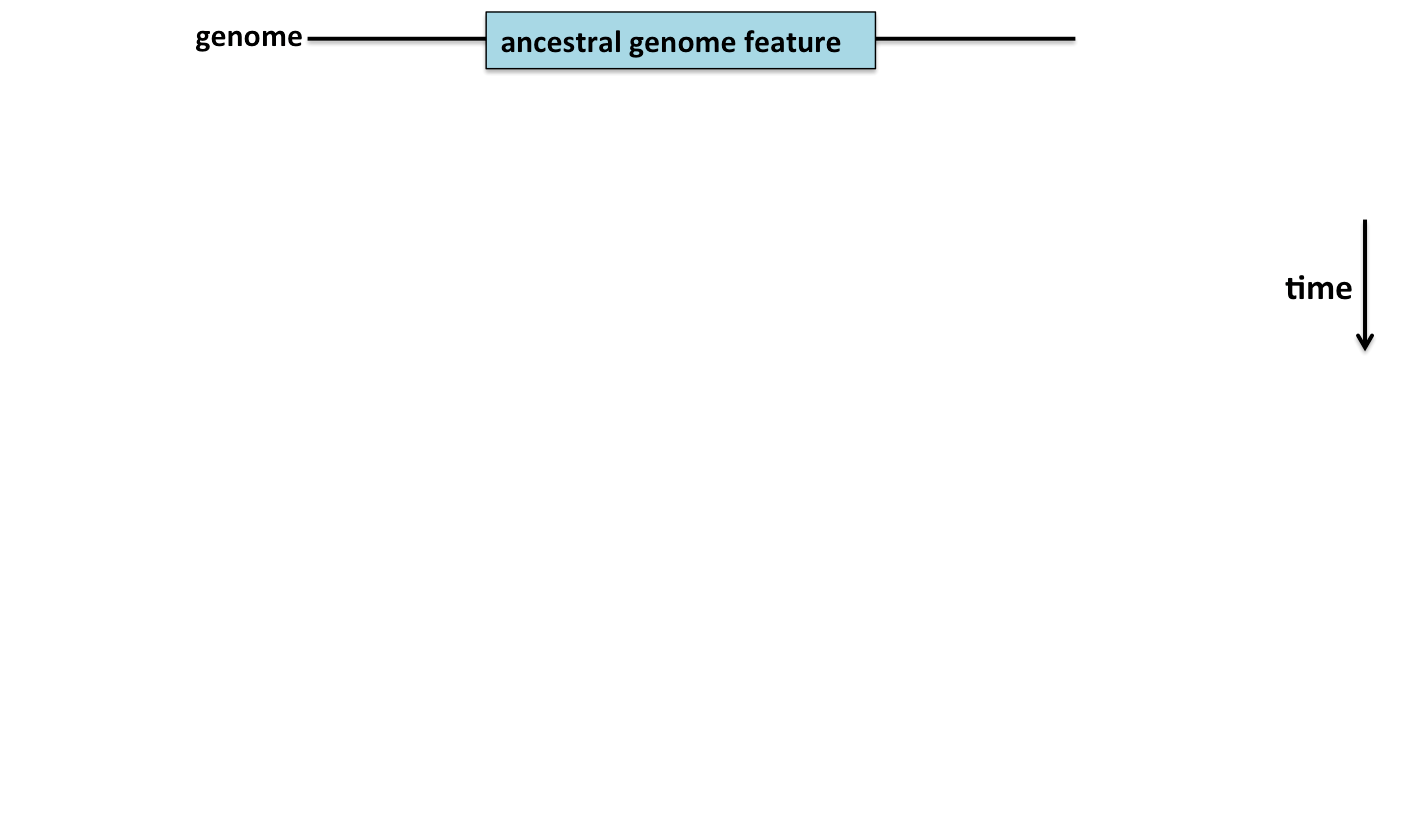
\includegraphics[width=1\textwidth]{images/logues1}  
  \end{center}  
\end{frame}

% Regulatory features
\begin{frame}
  \frametitle{Who let the -logues out?}
  \begin{center}
    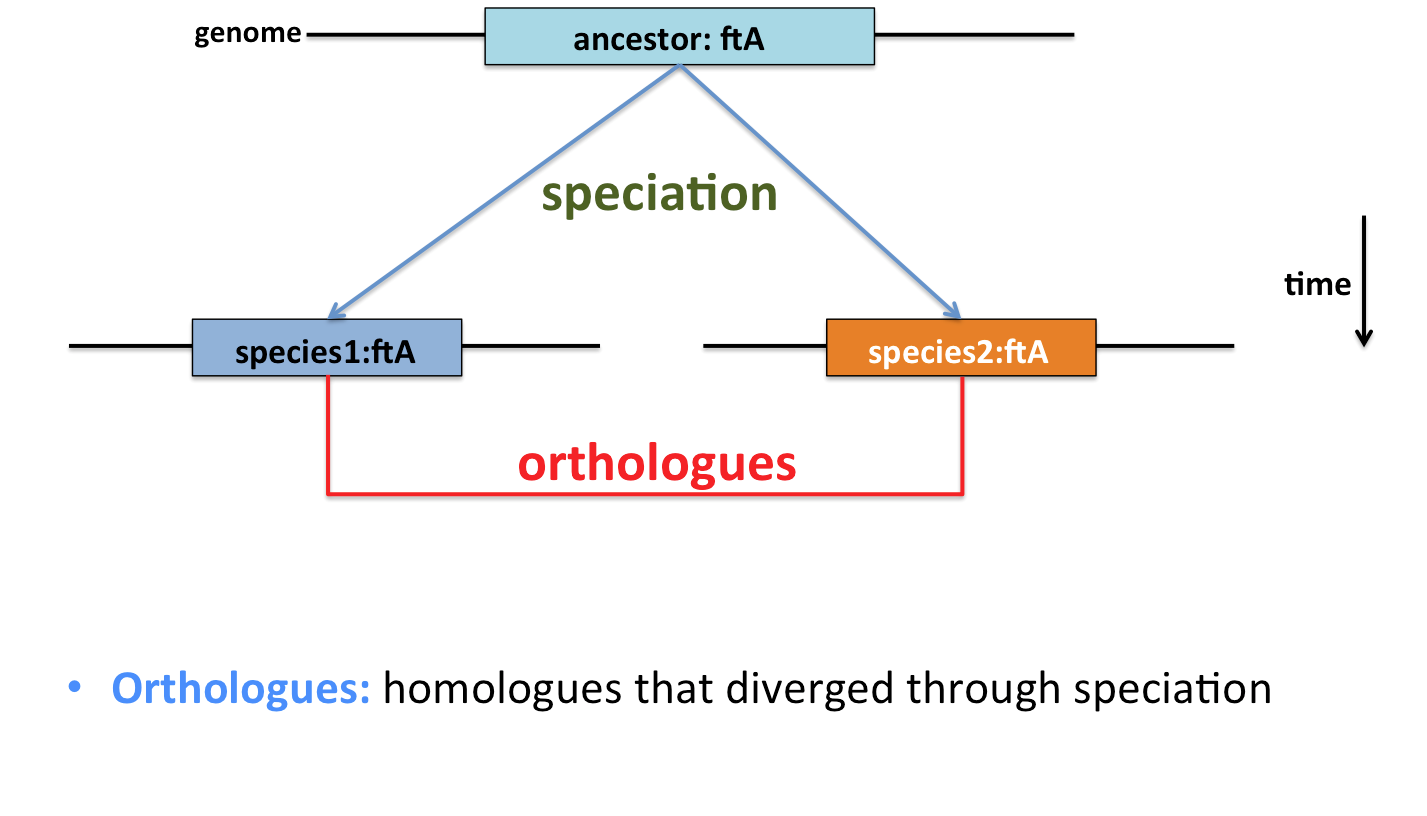
\includegraphics[width=1\textwidth]{images/logues2}  
  \end{center}  
\end{frame}

% Regulatory features
\begin{frame}
  \frametitle{Who let the -logues out?}
  \begin{center}
    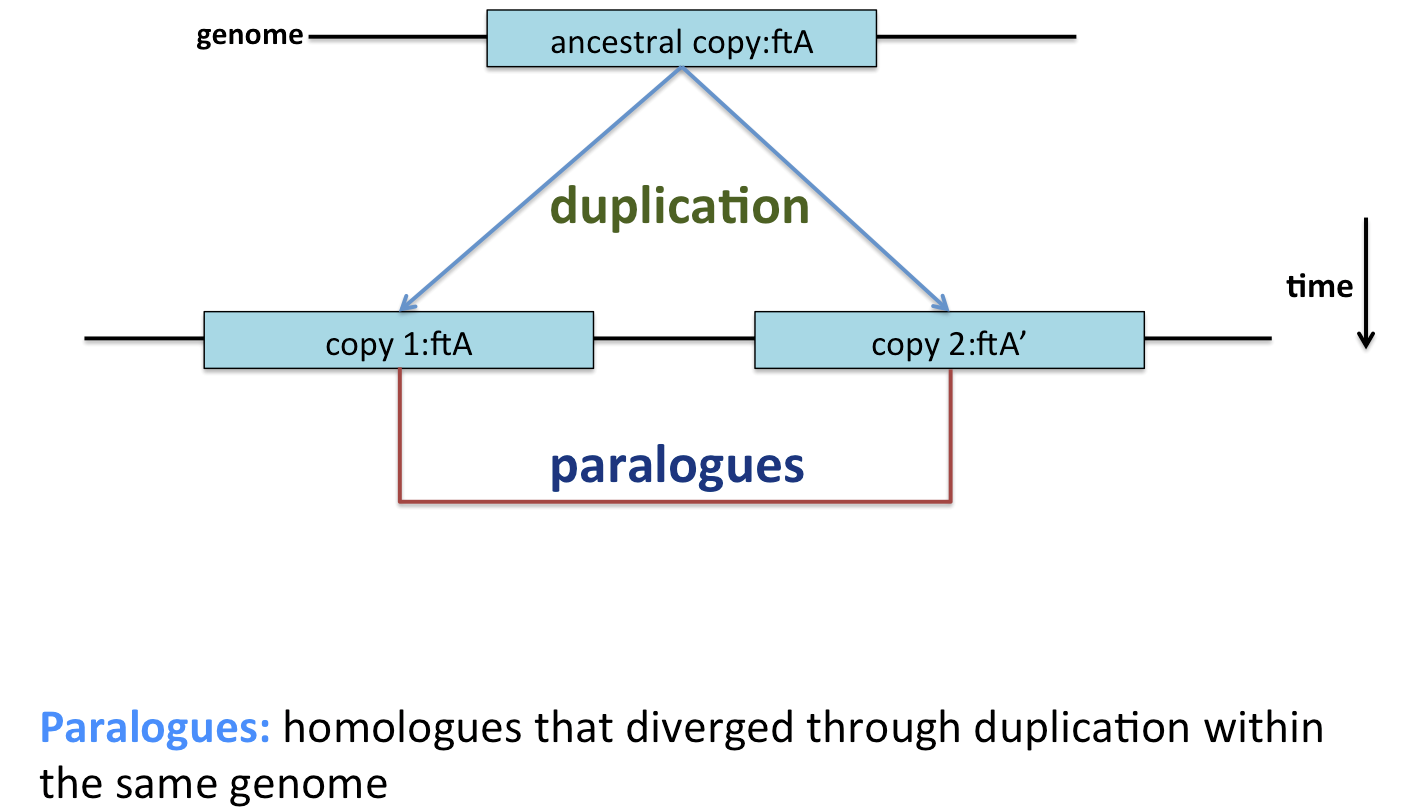
\includegraphics[width=1\textwidth]{images/logues3}  
  \end{center}  
\end{frame}

% Regulatory features
\begin{frame}
  \frametitle{Who let the -logues out?}
  \begin{center}
    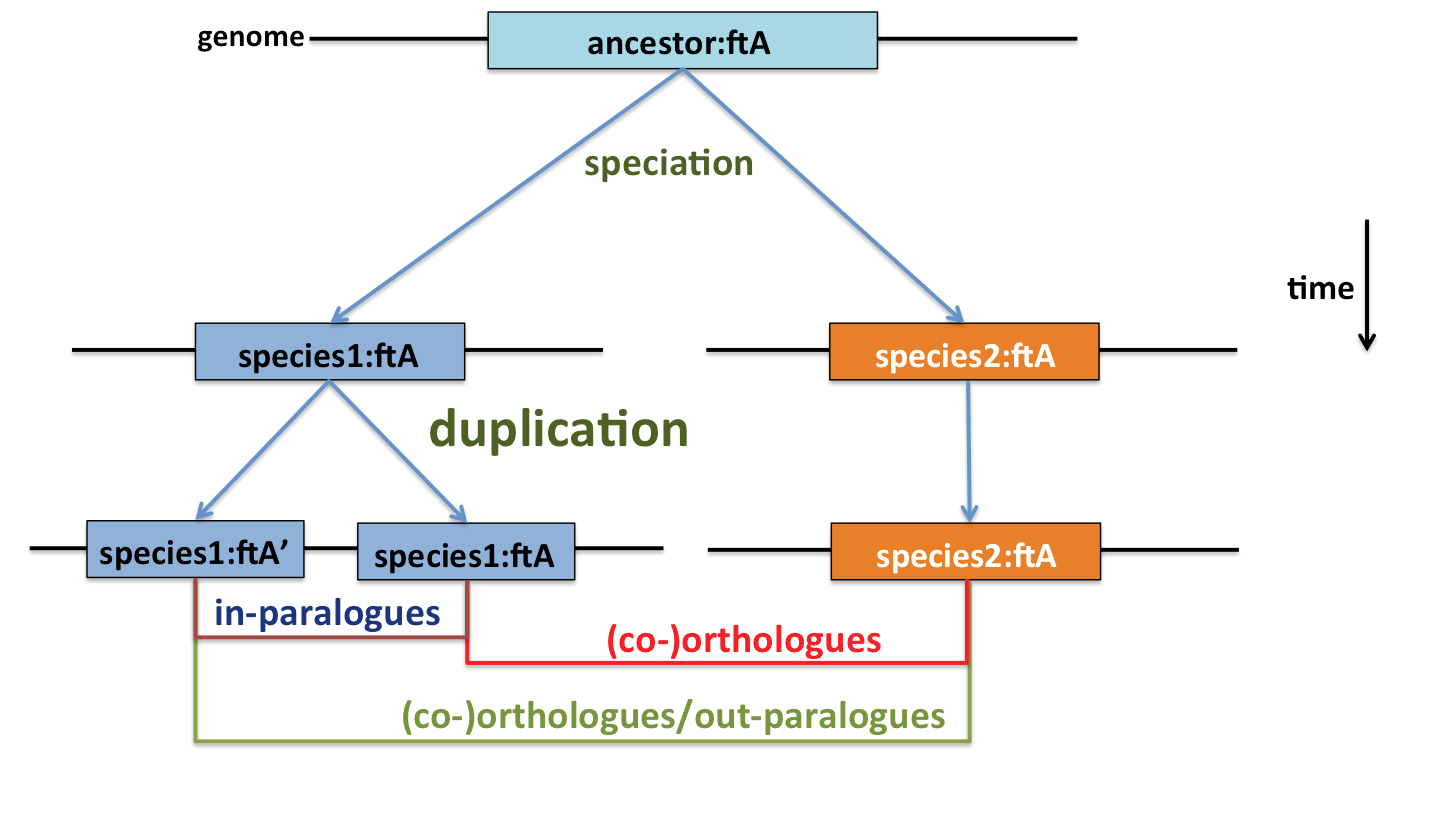
\includegraphics[width=1\textwidth]{images/logues4}  
  \end{center}  
\end{frame}

% Regulatory features
\begin{frame}
  \frametitle{Who let the -logues out?}
  \begin{center}
    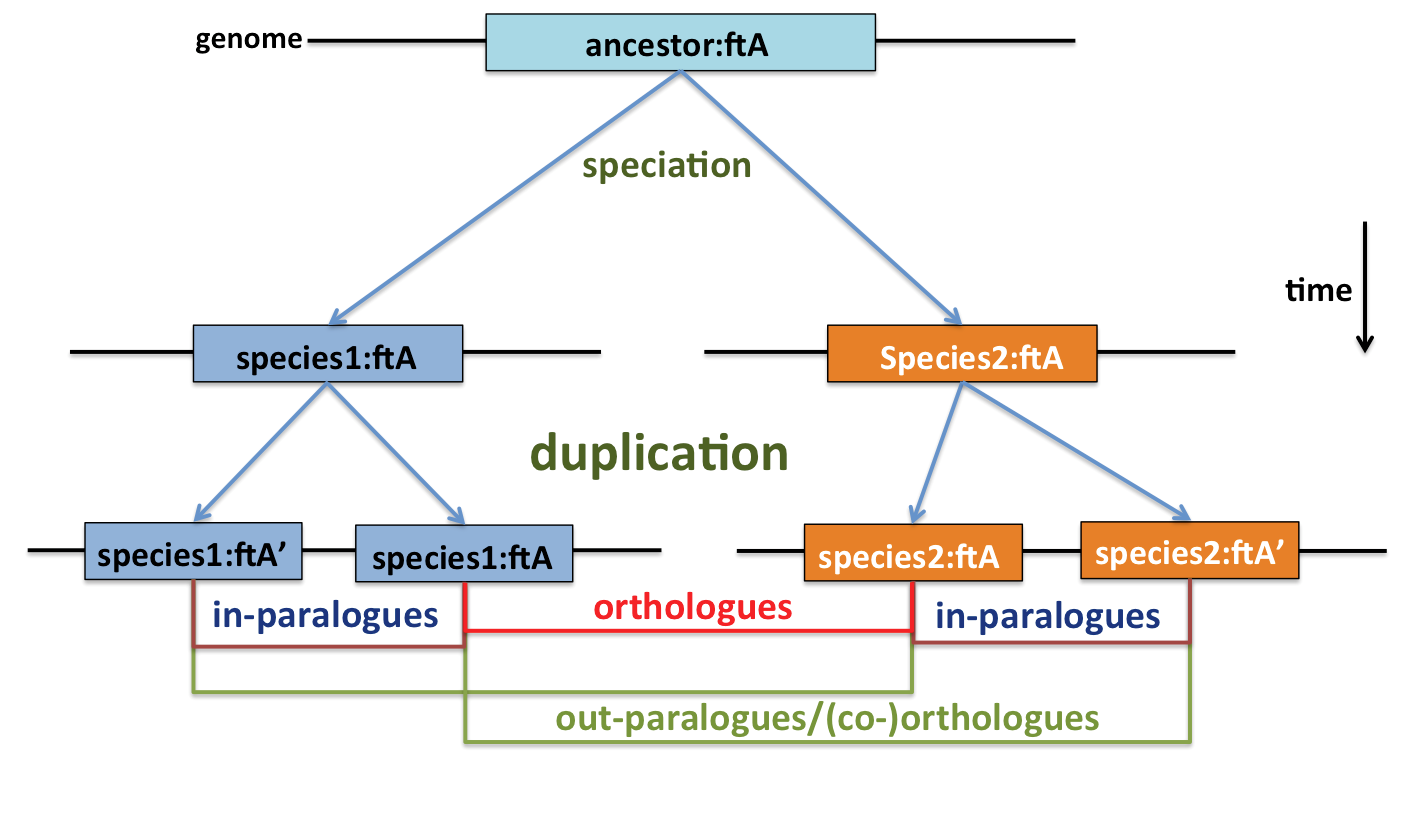
\includegraphics[width=1\textwidth]{images/logues5}  
  \end{center}  
\end{frame}

% Principles of feature prediction
\begin{frame}
  \frametitle{ITYFIALMCTT\footnote{\tiny{Kristensen \textit{et al}. (2011) \textit{Brief. Bioinf.} \textbf{12}:379-391 \href{http://dx.doi.org/10.1093/bib/bbr030}{doi:10.1093/bib/bbr030}}}}
  But it's a little more complicated than that. \\
  Biology is not well-behaved.
  \begin{itemize}
    \item Gene loss
    \item Homologues may diverge so widely that they can be hard to recognise
    \item Reconstructed evolutionary trees may not be robust inferences of speciation (or relevant to it, in prokaryotes)
    \item There is no record of history - we can only make inferences
  \end{itemize}
  \textbf{All classifications of orthology/paralogy are inferences!}
\end{frame}

% Principles of feature prediction
\begin{frame}
  \frametitle{ITYFIALMCTT\footnote{\tiny{Kristensen \textit{et al}. (2011) \textit{Brief. Bioinf.} \textbf{12}:379-391 \href{http://dx.doi.org/10.1093/bib/bbr030}{doi:10.1093/bib/bbr030}}}}
  \begin{center}
    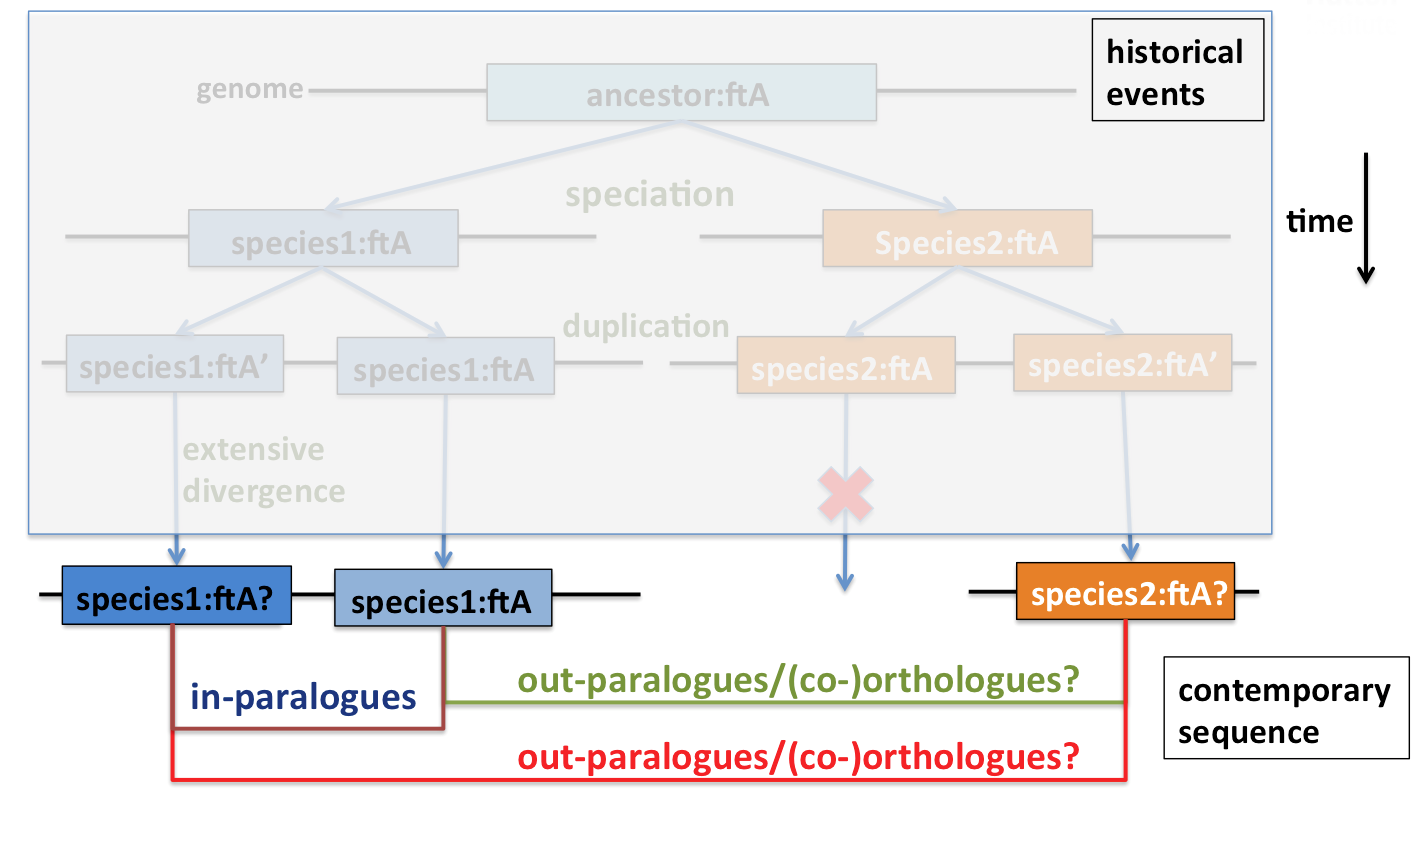
\includegraphics[width=1\textwidth]{images/logues6}  
  \end{center} 
  \textbf{All classifications of orthology/paralogy are inferences!}
\end{frame}

\begin{frame}
  \frametitle{Ensembl Compara\footnote{\tiny{Vilella \textit{et al}. (2009) \textit{Genome Res.} \textbf{19}:327-335 \href{http://dx.doi.org/10.1101/gr.073585.107}{doi:10.1101/gr.073585.107}}}}
  Some tools/databases, e.g. \href{http://www.ensembl.org/info/genome/compara/index.html}{Ensembl Compara}, use slightly different definitions (almost everything's an ``orthologue'')
  \begin{center}
    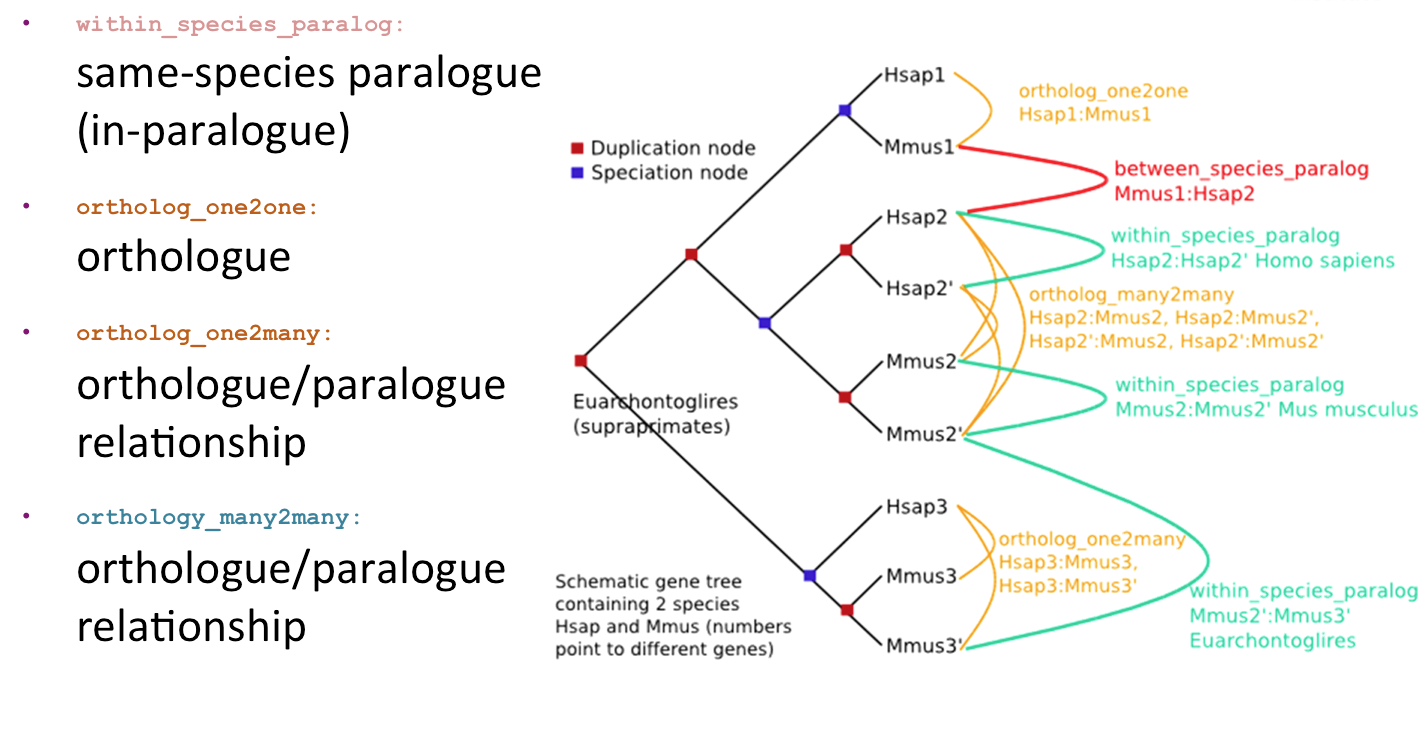
\includegraphics[width=1\textwidth]{images/logues7}  
  \end{center} 
\end{frame}